\documentclass[12pt,a4paper,oneside]{book}

\makeatletter
\newcommand\thefontsize[1]{{}}
\makeatother
\usepackage[utf8]{inputenc}
\usepackage{enumitem}
\usepackage{varwidth}
\usepackage{graphicx}
\usepackage{float}
\usepackage{caption}

\usepackage[top=2.5cm, bottom=3cm, left=2.5cm, right=2.5cm]{geometry}
\usepackage[utf8]{inputenc}
\usepackage[titletoc,title]{appendix}
\usepackage[linewidth=1pt]{mdframed}
\usepackage{framed}
\usepackage{listings}
\usepackage{smartdiagram}
\usepackage{smartdiagram}
\usepackage{varwidth}
\usepackage{amsmath}
\usesmartdiagramlibrary{additions}
\lstdefinestyle{customc}{
	belowcaptionskip=1\baselineskip,
	breaklines=true,
	frame=L,
	xleftmargin=\parindent,
	language=C,
	showstringspaces=false,
	basicstyle=\footnotesize\ttfamily,
	keywordstyle=\bfseries\color{green!40!black},
	commentstyle=\itshape\color{purple!40!black},
	identifierstyle=\color{blue},
	stringstyle=\color{orange},
}

\lstdefinestyle{customasm}{
	belowcaptionskip=1\baselineskip,
	frame=L,
	xleftmargin=\parindent,
	language=[x86masm]Assembler,
	basicstyle=\footnotesize\ttfamily,
	commentstyle=\itshape\color{purple!40!black},
}

\lstset{escapechar=@,style=customc}

\lstset{
	literate=%
	{à}{{\'a}}1
	{í}{{\'i}}1
	{é}{{\'e}}1
	{è}{{\`e}}1
	{ý}{{\'y}}1
	{ú}{{\'u}}1
	{ó}{{\'o}}1
	{ě}{{\v{e}}}1
	{š}{{\v{s}}}1
	{č}{{\v{c}}}1
	{ř}{{\v{r}}}1
	{ž}{{\v{z}}}1
	{ď}{{\v{d}}}1
	{ť}{{\v{t}}}1
	{ň}{{\v{n}}}1
	{ů}{{\r{u}}}1
	{Á}{{\'A}}1
	{Í}{{\'I}}1
	{É}{{\'E}}1
	{Ý}{{\'Y}}1
	{Ú}{{\'U}}1
	{Ó}{{\'O}}1
	{Ě}{{\v{E}}}1
	{Š}{{\v{S}}}1
	{Č}{{\v{C}}}1
	{Ř}{{\v{R}}}1
	{Ž}{{\v{Z}}}1
	{Ď}{{\v{D}}}1
	{Ť}{{\v{T}}}1
	{Ň}{{\v{N}}}1
	{Ů}{{\r{U}}}1
}

\begin{document}

	\tableofcontents

	\listoffigures

	
	\chapter{Introduction }
	bla bla for tp and le but of ir
	\chapter{Réalisation}
	\section{L'outil cygwin}
	  why did we use it and all
	\section{Étape 1:}
	\subsection{Utilisation du prod1vid.m}
	 principalement prod1vid construit un réseau causal probabiliste basé sur le produit tel que les connexions entre les nœuds sont aléatoires , ainsi que les valeurs initiales attribués à la variable d'intérêt et l'évidence .
	 Pour exécuter le programme il faut:
	 \begin{itemize}
	 	\item sur Matlab taper : prod1vid
	 	
	 \end{itemize}
	 ce que le programme offre en sortie est environnement ou on peut voir toutes les variables et le graphe (matrice) crée.
	 on peut alors afficher :
	 
	 \begin{itemize}
	 	\item la variable d'intérêt sachant l'évidence
	 	\item temps de la propagation
	 	\item type de graphe (multi-connected (multi-connectés) ou polytree (polyarbre))
	 \end{itemize}
	 \subsubsection{Fonctionnement du programme}
	 Aprés avoir étudier le programme on a pu résumer son fonctionnement dans les étapes qui suivent :
	 \begin{enumerate}
	 	\item Initialisation du nombre de parents max globale et nombre de noeuds du graphe à construire
	 	\item Création de liens de façon aléatoire entre les noeuds.
	 	\item Utilisation de processus de fixation après la création aléatoire afin d'éviter les noeuds isolés et sous graphes isolés ( les inconvénients de l'aléatoire)
	 	\item Prise de considération des domaines des variables (représentés par les noeuds)
	 	cas binaire etc ...
	 	\item Génération de la distribution aléatoire initiale du graphe crée (de possibilité initiales).
	 	\item génération aléatoire d'une évidence  : une évidence est une information nouvelle qui viens et à qui on aimerait calculer l'influence qu'elle aura sur la variable d'intérêt(évidente est comme une condition ).
	 	\item Détermination si le graphe est polytree ou multi-connected
	 	\item Lancement de la propagation ( algorithme de propagation)
	 	
	 	
	 \end{enumerate}
	 
	 Concernant \textbf{Prodevid2} c'est le mème fonctionnement à part qu'on a droit à deux évidences donc deux informations vont influer notre réseau , en théorie  on peut penser que la propagation des deux évidences prendra plus de temps que celle d'une seule , on testera ce cas dans ce qui suit .
	 
	
	\subsection{Réglage de paramètres}
	\subsubsection{Jeu de test}
	On a choisi de fixer le nombre de noeuds à :10
	
	et le nombre de parent max à :2 
	
	ce qui est censé nous donnée un polytree .
	\subsubsection{Code}
	
    	\begin{figure}[h]
		\centering
		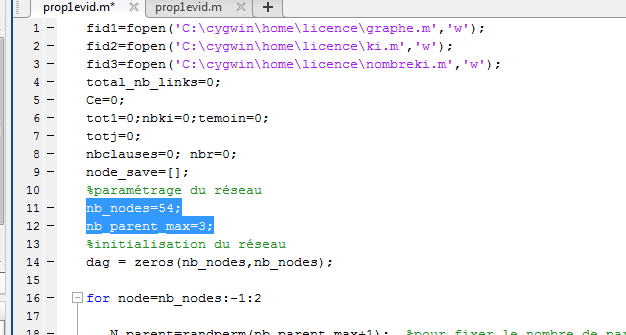
\includegraphics[scale=0.7]{screens/prodevid1code.png}
		\captionof{figure}{Le changement des nb noeuds ainsi que nb parents max dans le code prod1evid.m}\label{labelname}%
		\end{figure}
	
	On a choisi de fixer \textbf{le nombre de nœuds à : 54}
	
	et \textbf{le nombre de parents max à :3 }
	
   \paragraph{Remarque}
   Dans le code fourni Pour avoir le nombre de parents d'un nœud , le programme tire aléatoirement un nombre entre \textbf{[1,nbparentsmax+1]} donc concrètement  le nombre de parents max est de 4 et non de 3  voir code:prod1evid.m.
   
	\subsubsection{Affichage}
	le résultat était le suivant :
	
	
	\begin{frame}{}
		\centering
		\begin{minipage}[H]{0.5\linewidth}
			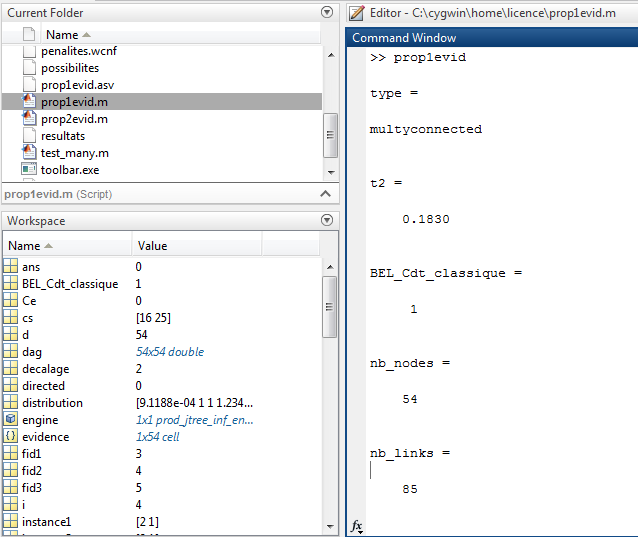
\includegraphics[width=1\textwidth]{screens/prodevid1affichge.png}%
			\captionof{figure}{Une seule evidence}\label{labelname}%
		\end{minipage}
		\hspace{0.5cm}
		\begin{minipage}[H]{0.5\linewidth}
			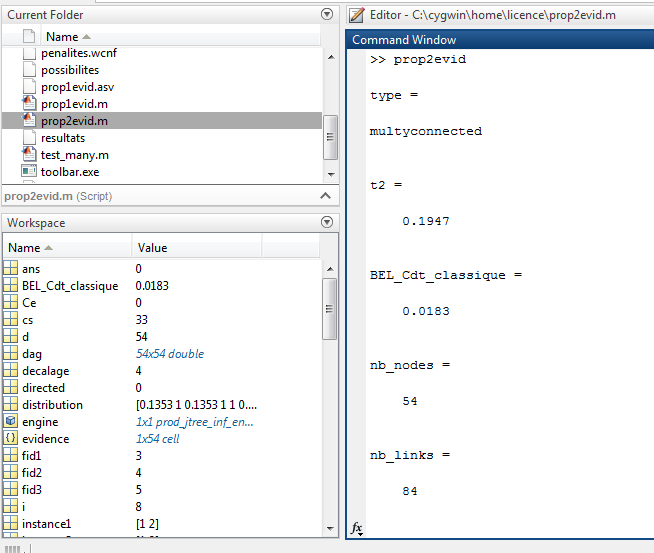
\includegraphics[width=1\textwidth]{screens/prodevid2affichage.png}%
			\captionof{figure}{Deux evidences}\label{labelname}%
		\end{minipage}
	\end{frame}

		\begin{center}
			\begin{tabular}{ | l || c | c | }
				\hline
				\textbf{nombre d'évidence} & 1 &  2\\
				\hline
				\textbf{temps de propagation} & 0.18 secondes & 0.19 secondes\% \\
				\hline
				\textbf{Bel variable d'intérêt} & 1 & 0.018 \\
				\hline
			\end{tabular}
		\end{center}

		
	\subsubsection{Explication et observation}
    	Comme on a pu le deviner la propagation prend plus de temps avec deux évidences qu'avec une seule , car le calcul des nouvelles distributions de possibilités est plus complexe avec deux informations qui arrivent qu'avec une seule .
	
	\section{Étape 2}
	\subsection{Explication  }
      Dans cette étape il nous ai demandé d'utiliser deux programmes exécutables
      à fin de passer d'une modélisation graphique avec des algorithmes de propagation à une une représentation logique en clauses (max sat weighted ) en utilisant le processus d'inférence.
            Prodevid1 donne en sortie un graphe ( matrice en matlab) qui modélise le graphe crée
            \begin{figure}[H]
            	\centering
            	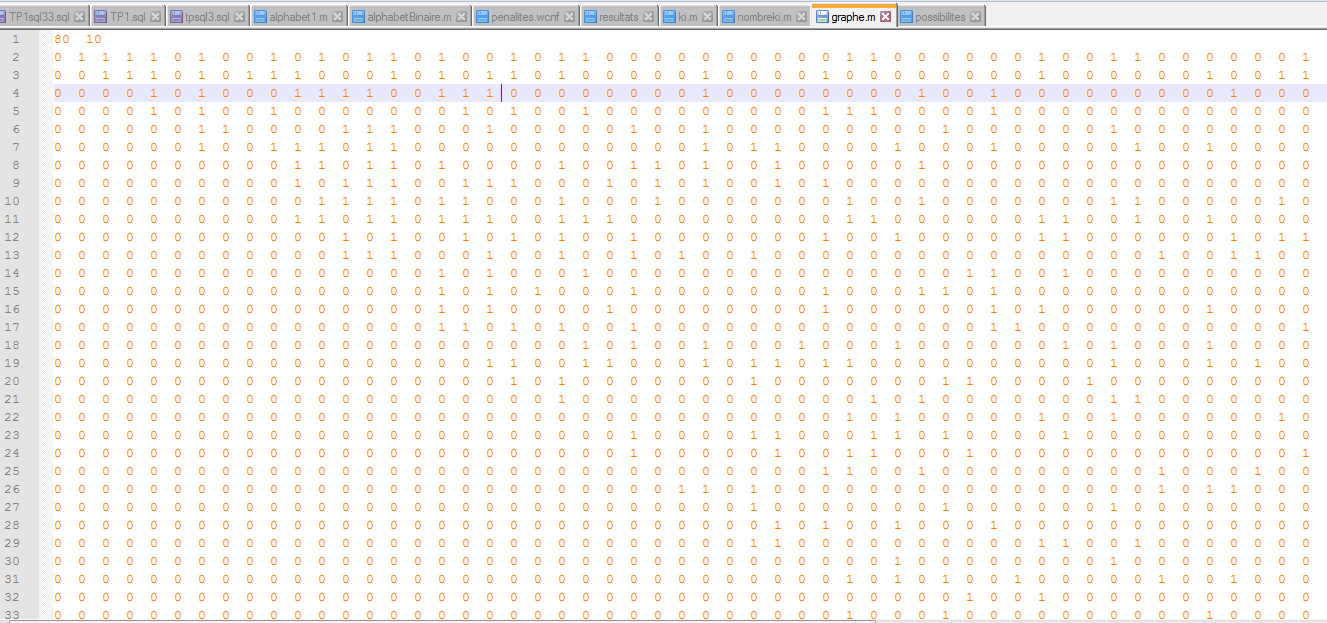
\includegraphics[scale=0.7]{screens/etape2graph.png}
            	\captionof{figure}{exemple d'un graphe en sortie à l'éxecution de  prod1evid.m avec noeuds=80 et parents =10}\label{labelname}%
            	
            \end{figure}
            \begin{figure}[H]
            	\centering
            	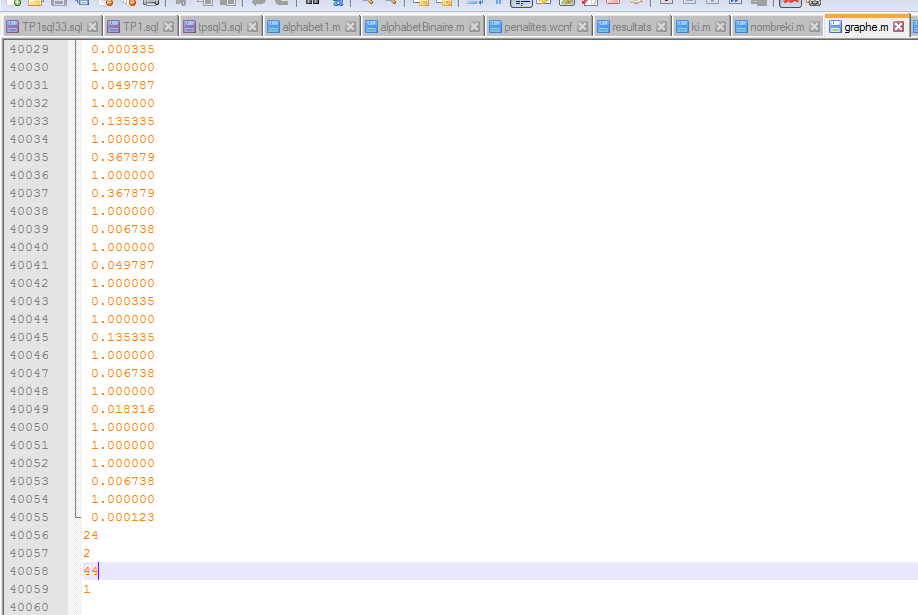
\includegraphics[scale=0.7]{screens/etape2graph2.png}
            	\captionof{figure}{exemple d'un graphe en sortie à l'éxecution de  prod1evid.m avec noeuds=80 et parents =10}\label{labelname}%
            \end{figure}
      
      Tout d'abord on reprend l'exemple vu dans l'étape 1 avec un nombre de noeuds à 54 et nombre de parents max à 4 puis il faudra faire :
      \begin{itemize}
      	\item Se placer dans le dossier licence sous terminal de cygwin .
      	\item Exécuter le prod1evid sous matlab
      	\item Exécuter le ./passage.exe qui convertit les graph.m en clauses (maxSat)
      	\item Lancement du processus d'inférence on aura le temps de l'inférence en MICRO SECONDES.
      	\item Affichage du résultat avec la commande : cat résultats
      \end{itemize}
      
      \subsubsection{Affichage}
      
      
      
      	
      		\begin{figure}[H]
      				\centering
      			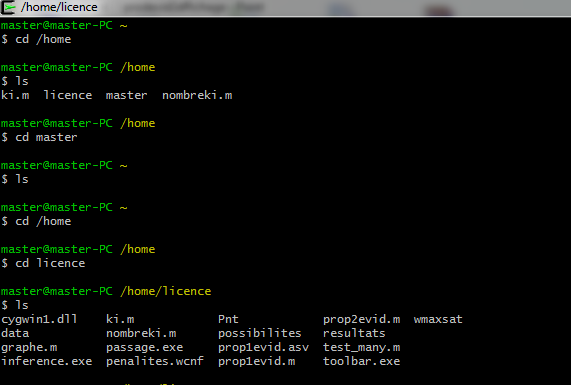
\includegraphics[scale=1]{screens/etape2terminal.png}%
      			\captionof{figure}{Les commandes necessaires pour lancer l'inference}\label{labelname}%
      		\end{figure}
      		
      		\begin{figure}[H]
      				\centering
      			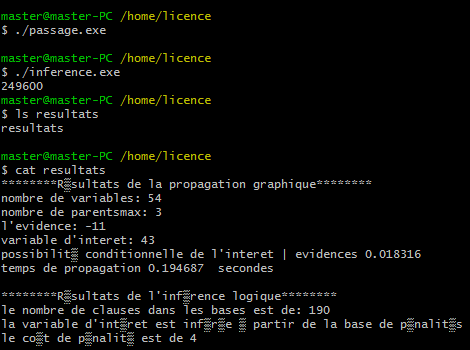
\includegraphics[scale=1.1]{screens/etape2.png}%
      			\captionof{figure}{Lancement de passage et inference }\label{labelname}%
      		\end{figure}
        
        
        \subsubsection{Observation}
        on remarque dans notre cas on à affaire à un réseau multi-connected on a remarqué que la propagation était prenait presque autant de temps que l'inférence , on peut expliquer ça par le fait qu'on manipule des graphes où le nombres de noeuds et connexions n'est pas conséquent par contre dans le cas ou le nombre de noeuds était 80 et parents = 10 la propagation avait pris beaucoup plus de temps  voir l'etape 3 comparé à l'inférence qui fait appel à un solver max sat .

       
    \section{Etape 3}
    \subsection{Géneration automatique aléatoire des Graphes}
    \subsubsection{Géneration des Polytree(youpii)}
    \subsubsection{Géneration des Multiconnected}
    \subsubsection{Géneration des simplement connected}
    \section{Résultats}
    
    \section{Observation pour chaque type }
    \section{Observation et comparaison entre les differents types}

\end{document}